\documentclass[a4paper,12pt]{article}
\usepackage{graphicx}
\usepackage{amsmath}
\usepackage{float}
\usepackage{setspace}
\usepackage[margin=1in]{geometry}
\usepackage{caption}

\title{\textbf{Is Florida Getting Warmer?}}
\author{Yijia Yao}
\date{}

\begin{document}

\maketitle
\doublespacing

\section*{Introduction}
Global climate change is one of the most pressing environmental issues of our time.
To understand how global warming manifests regionally, we analyze temperature data from Key West, Florida, covering the entire 20th century (1901–2000). 
The goal is to determine whether there is a statistically significant warming trend over this period.

Because annual temperature measurements are temporally correlated, standard correlation tests assuming independent observations may not be appropriate. 
To address this, we use a permutation test to estimate the significance of the correlation between temperature and year.

\section*{Methods}
The dataset (\texttt{KeyWestAnnualMeanTemperature.RData}) contains two columns: \texttt{Year} and \texttt{Temp}.
We first computed the Pearson correlation coefficient ($r$) between year and annual mean temperature.
Then, we generated a null distribution of correlation coefficients by randomly permuting the temperature values 10,000 times using the \texttt{sample()} function in R, while keeping the years fixed.

Each permutation breaks any temporal structure, representing the null hypothesis of no temporal trend.
The permutation p-value was calculated as the fraction of permuted $r$ values greater than or equal to the observed correlation coefficient.

\section*{Results}
The observed correlation coefficient between year and temperature was:
\[
r_{\text{observed}} = 0.53
\]
This positive correlation suggests that temperature has increased over time in Key West.

To evaluate statistical significance, we compared this value against the permutation-based null distribution of 10,000 random correlations. 
Only about 0.3\% of the permuted correlations were greater than the observed value, giving an approximate p-value of $p = 0.003$.

\begin{figure}[H]
    \centering
    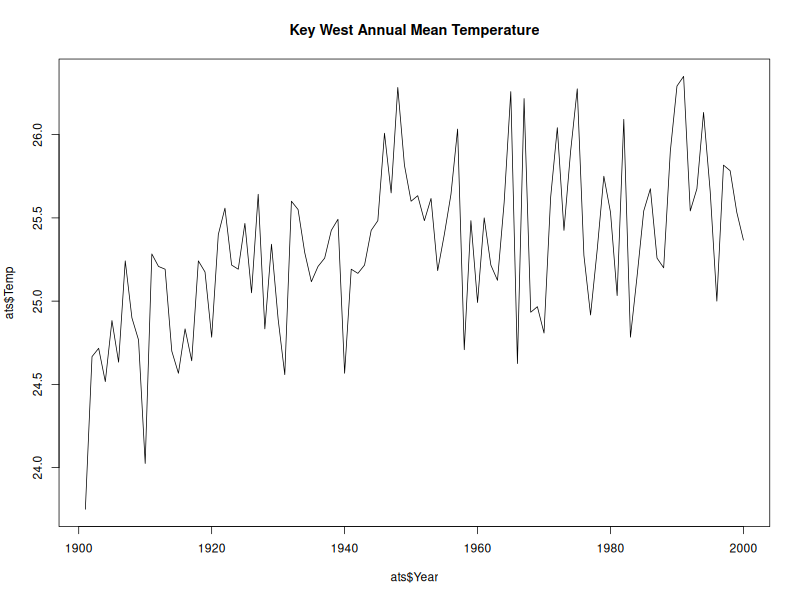
\includegraphics[width=0.85\linewidth]{Florida_TempTrend.png}
    \caption{Annual mean temperature in Key West, Florida (1901–2000). A clear upward trend is visible over the century.}
\end{figure}

\begin{figure}[H]
    \centering
    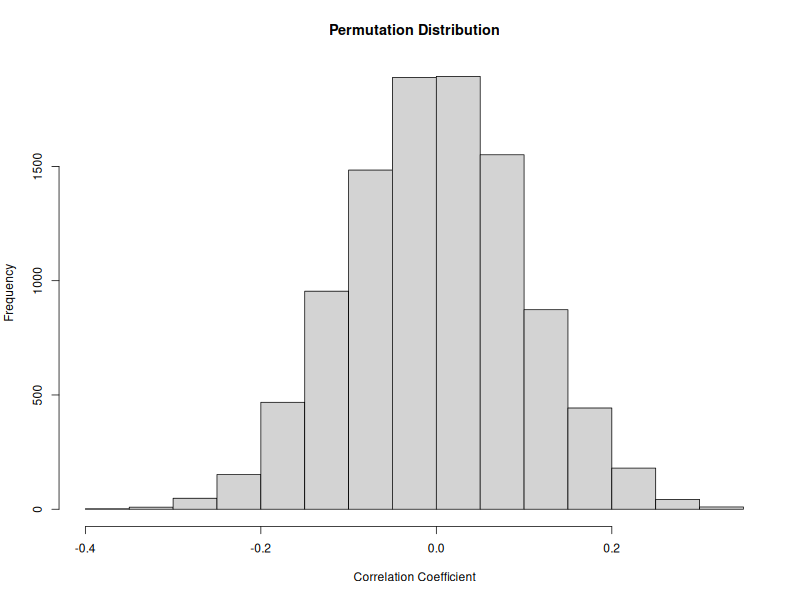
\includegraphics[width=0.85\linewidth]{Florida_PermutationDist.png}
    \caption{Null distribution of correlation coefficients from 10,000 permutations. The red dashed line marks the observed $r = 0.53$.}
\end{figure}

\section*{Discussion}
The permutation analysis confirms that the warming trend observed in Key West throughout the 20th century is statistically significant ($p < 0.01$). 
This result supports the hypothesis that Florida’s climate has become warmer over time.

While this simple correlation analysis does not account for other factors such as oceanic oscillations, urbanization, or measurement changes, the consistent positive trend is in line with broader regional and global warming patterns.

\section*{Conclusion}
Our analysis shows a strong and statistically significant warming trend in Key West, Florida, over the 20th century.
The permutation test confirms that this pattern is unlikely to have occurred by random chance.

\vspace{1em}
\noindent\textbf{Code and Data Availability:}  
All analyses were conducted in R using the dataset \texttt{KeyWestAnnualMeanTemperature.RData}.  
Figures were generated by the accompanying script \texttt{Florida.R} and saved automatically in the \texttt{week4/results/} directory.

\end{document}
